\documentclass[a4paper, 12pt, brazilian]{article}
\usepackage{config}

\title{FA576 - Prova}
\author{Renan da Silva Guedes \and RA: 223979}
\date{\today}

\begin{document}
	\maketitle
	\begin{itemize}
		\item[\textbf{(1)}] As duas equações que relacionam carga e deformação da lei de Hooke Generalizada são, respectivamente
		
		\begin{equation}
			\sigma_{ij}=\dfrac{E}{1+\nu}\left(\epsilon_{ij}+\dfrac{\nu}{1-2\nu}\,\delta_{ij}\,\epsilon_{kk}\right)
		\end{equation}
		
		\begin{equation}
			\epsilon_{ij}=\dfrac{1+\nu}{E}\,\sigma_{ij}-\dfrac{\nu}{E}\,\delta_{ij}\,\sigma_{kk}
		\end{equation}
		
		onde $\sigma_{ij}$
		
		\item[\textbf{(2)}] Esquemas
		
		\begin{figure}[H]
			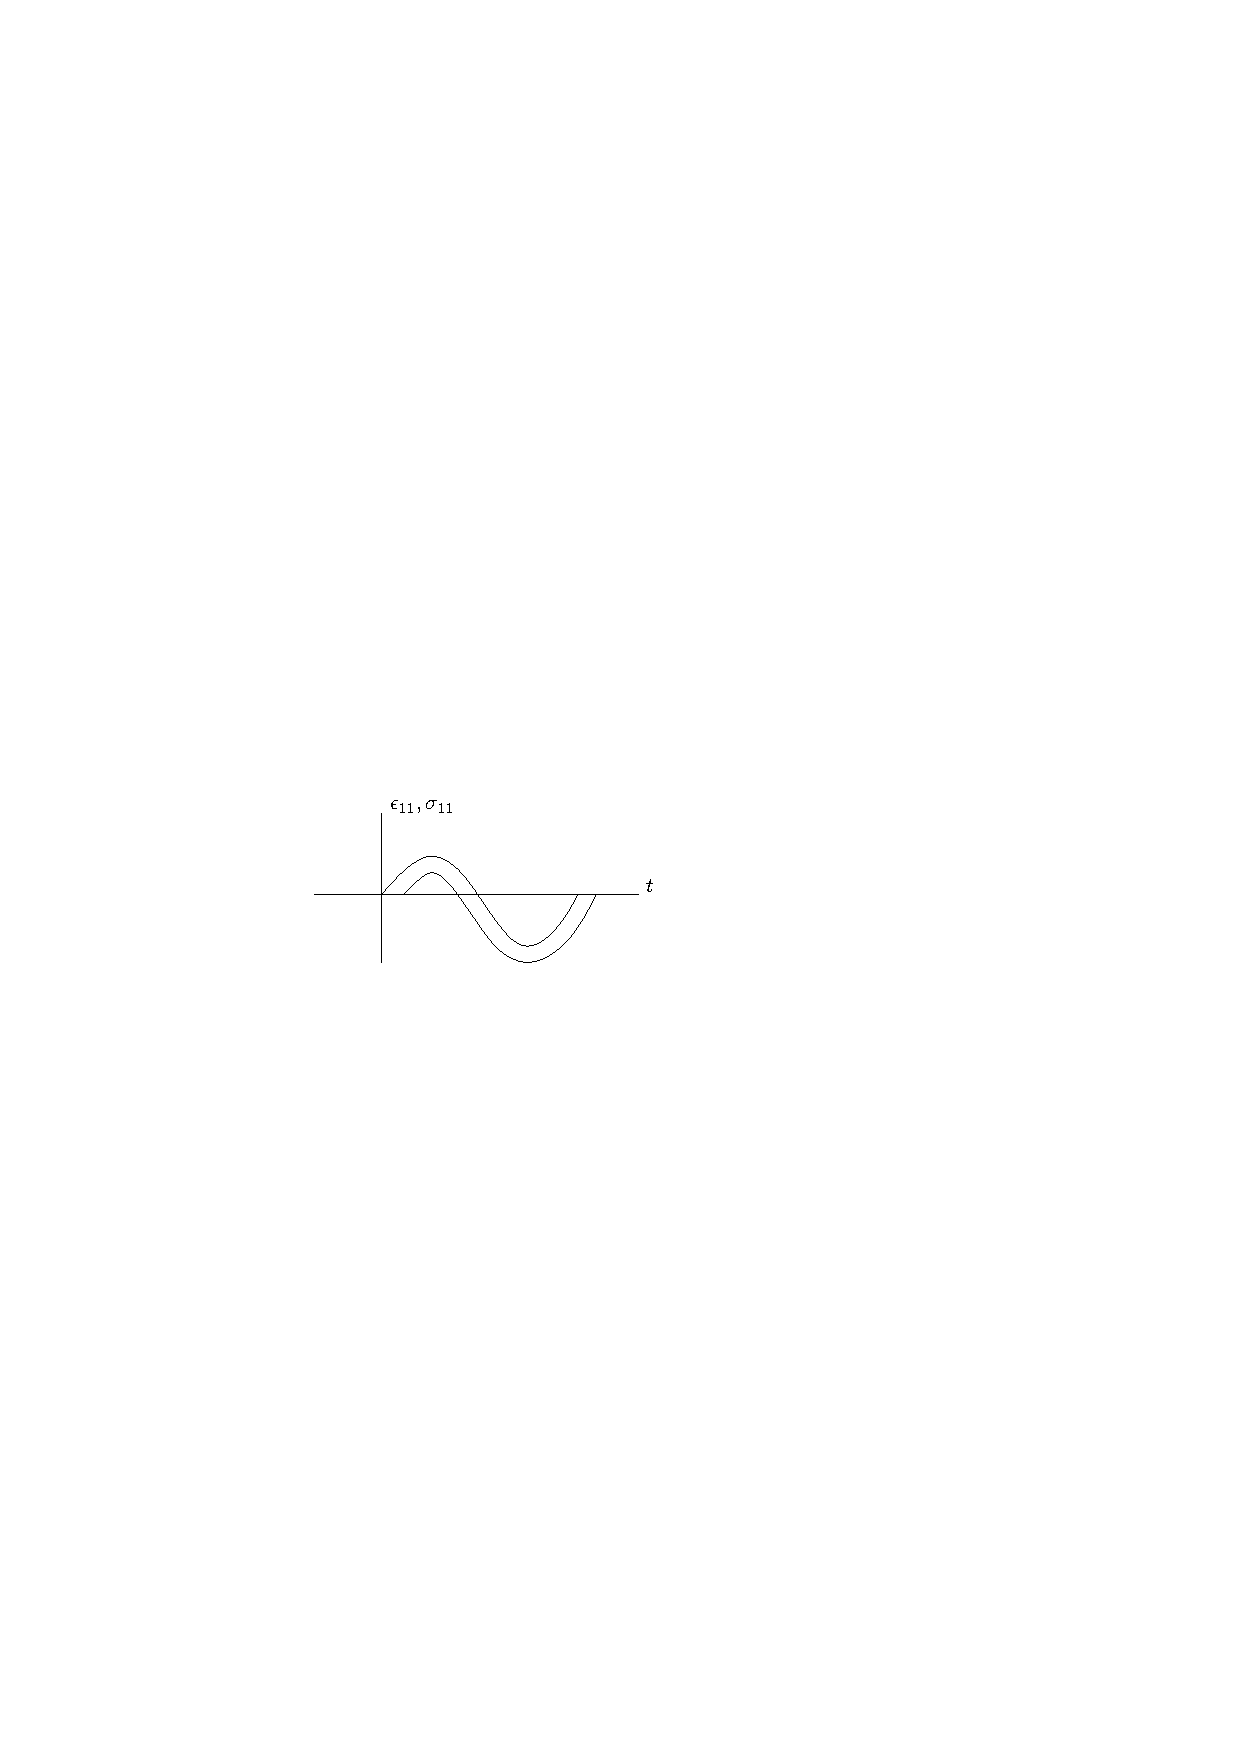
\includegraphics[scale=1.3]{images/elast}
			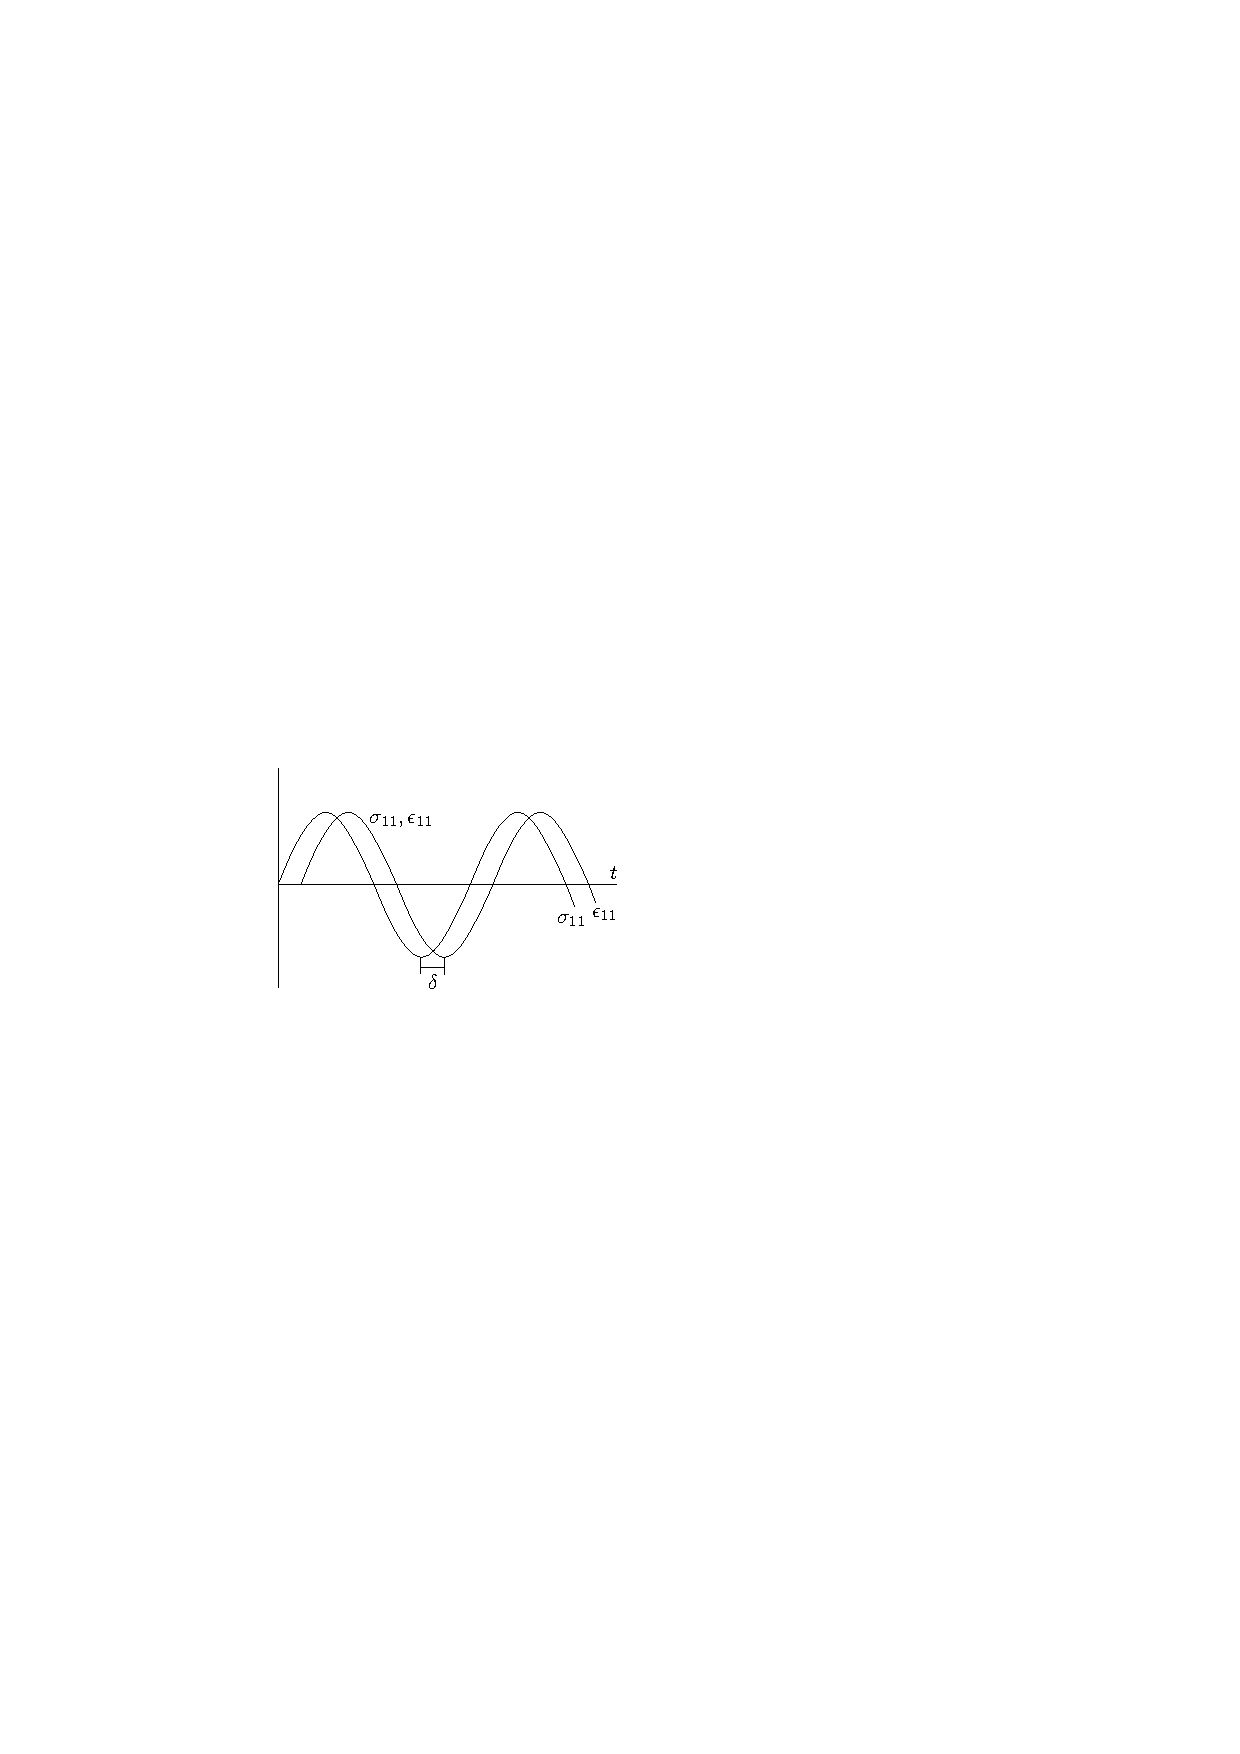
\includegraphics[scale=1.3]{images/inelast}
			\caption{Gráfico à direita ilustrando a resposta ao carregamento em um material viscoelástico, enquanto que à esquerda, elástico.}
		\end{figure}
		
		\item[\textbf{(4)}]
		
		\begin{itemize}
			\item[\textbf{(a)}] Na equação \eqref{eq:1} abaixo, a deformação em $i$ e $j$ dadas como função de $t$ representa o \textit{strain} total. O termo $d\sigma_{ij}(t')/dt'$ representa o \textit{strees rate}, onde $\sigma_{ij}$ é o tensor $\textit{stress}$. Por fim, o termo $\psi(t-t')$ denota a função \textit{creep}.
			
			\begin{equation}
				\label{eq:1}
				\epsilon_{ij}(t)=\int\limits_{0}^{t}\dfrac{d\sigma_{ij}(t')}{dt'}\,\psi(t-t')dt'
			\end{equation}
			
			Ao subdividir os tensores em hidrostáticos e deviatóricos duas funções viscoelásticas seriam envolvidas como segue
			
			\begin{equation}
				e_{ij}(t)=\int\limits_{0}^{t}\dfrac{ds_{ij}(t')}{dt'}\,\psi_{d}(t-t')dt'
			\end{equation}
			
			\begin{equation}
				\epsilon_{kk}(t)=\int\limits_{0}^{t}\dfrac{d\sigma_{kk}(t')}{dt'}\,\psi_{H}(t-t')dt'
			\end{equation}
			
			Análogo ao primeiro item, duas funções seriam obtidas como é visto em 
			
			\begin{equation}
				S_{ij}(t)=\int\limits_{0}^{t}\dfrac{de_{ij}(t')}{dt'}\,\phi_{d}(t-t')dt'
			\end{equation}
			
			\begin{equation}
				\sigma_{kk})(t)=\int\limits_{0}^{t}\dfrac{d\epsilon_{kk}(t')}{dt'}\,\phi_{H}(t-t')dt'
			\end{equation}
			
			\item[\textbf{(b)}] Na equação \eqref{eq:2} o termo $\sigma_{ij}$ é a função \textit{stress} total dependente do tempo. O termo $d\epsilon_{ij}(t')/dt'$ é a taxa de deformação (\textit{strain rate}), onde $\epsilon_{ij}$ é o tensor \textit{strain}. A função $\phi$ é \textit{relaxation}.
			
			\begin{equation}
				\label{eq:2}
				\sigma_{ij}(t)=\int\limits_{0}^{t}\dfrac{d\epsilon_{ij}(t')}{dt'}\,\phi(t-t')dt'
			\end{equation}
		\end{itemize}
	
		
	
		\begin{figure}[H]
			\centering
			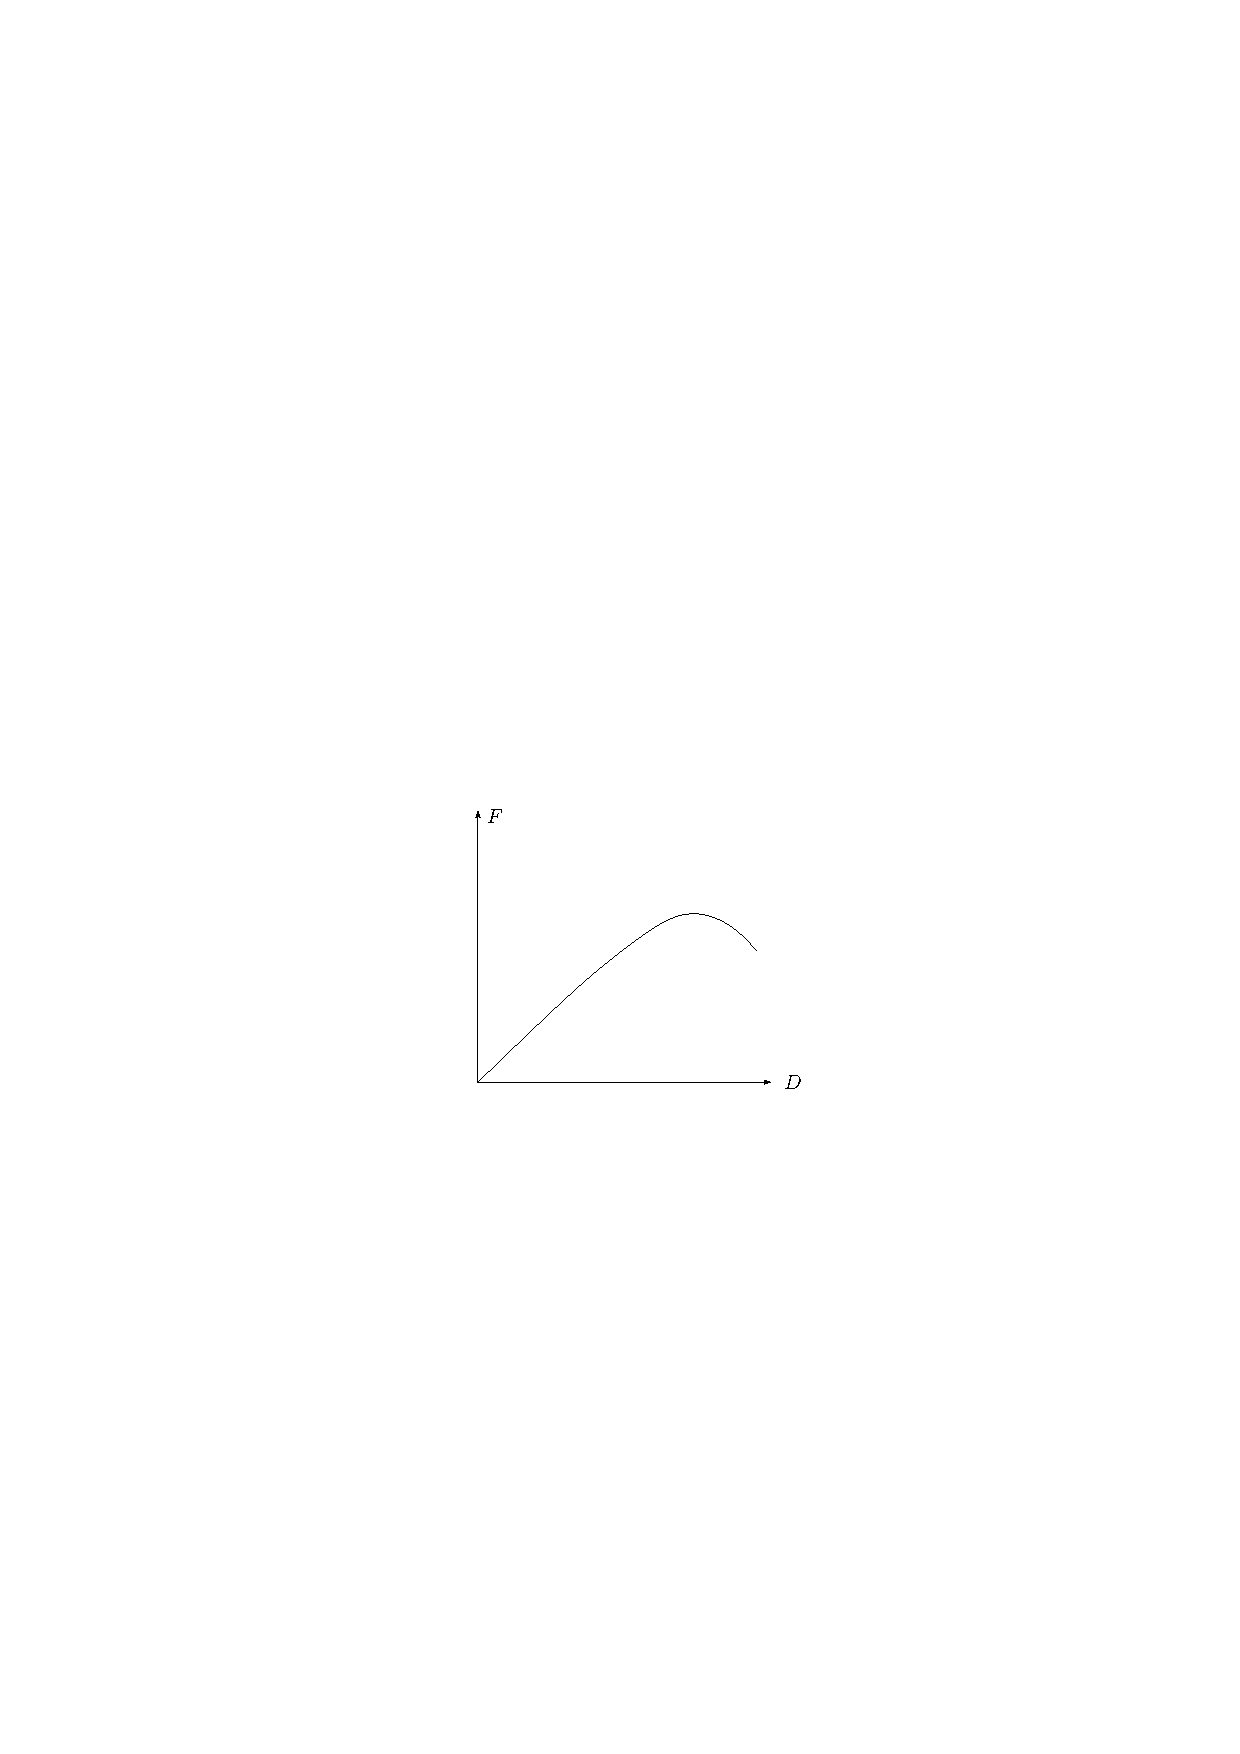
\includegraphics[scale=1.1]{images/brazilian}
		\end{figure}
	
		\item[\textbf{(6)}]	
		
		\begin{itemize}
			\item Modelo de Maxwell	
			\begin{figure}[H]
				\centering
				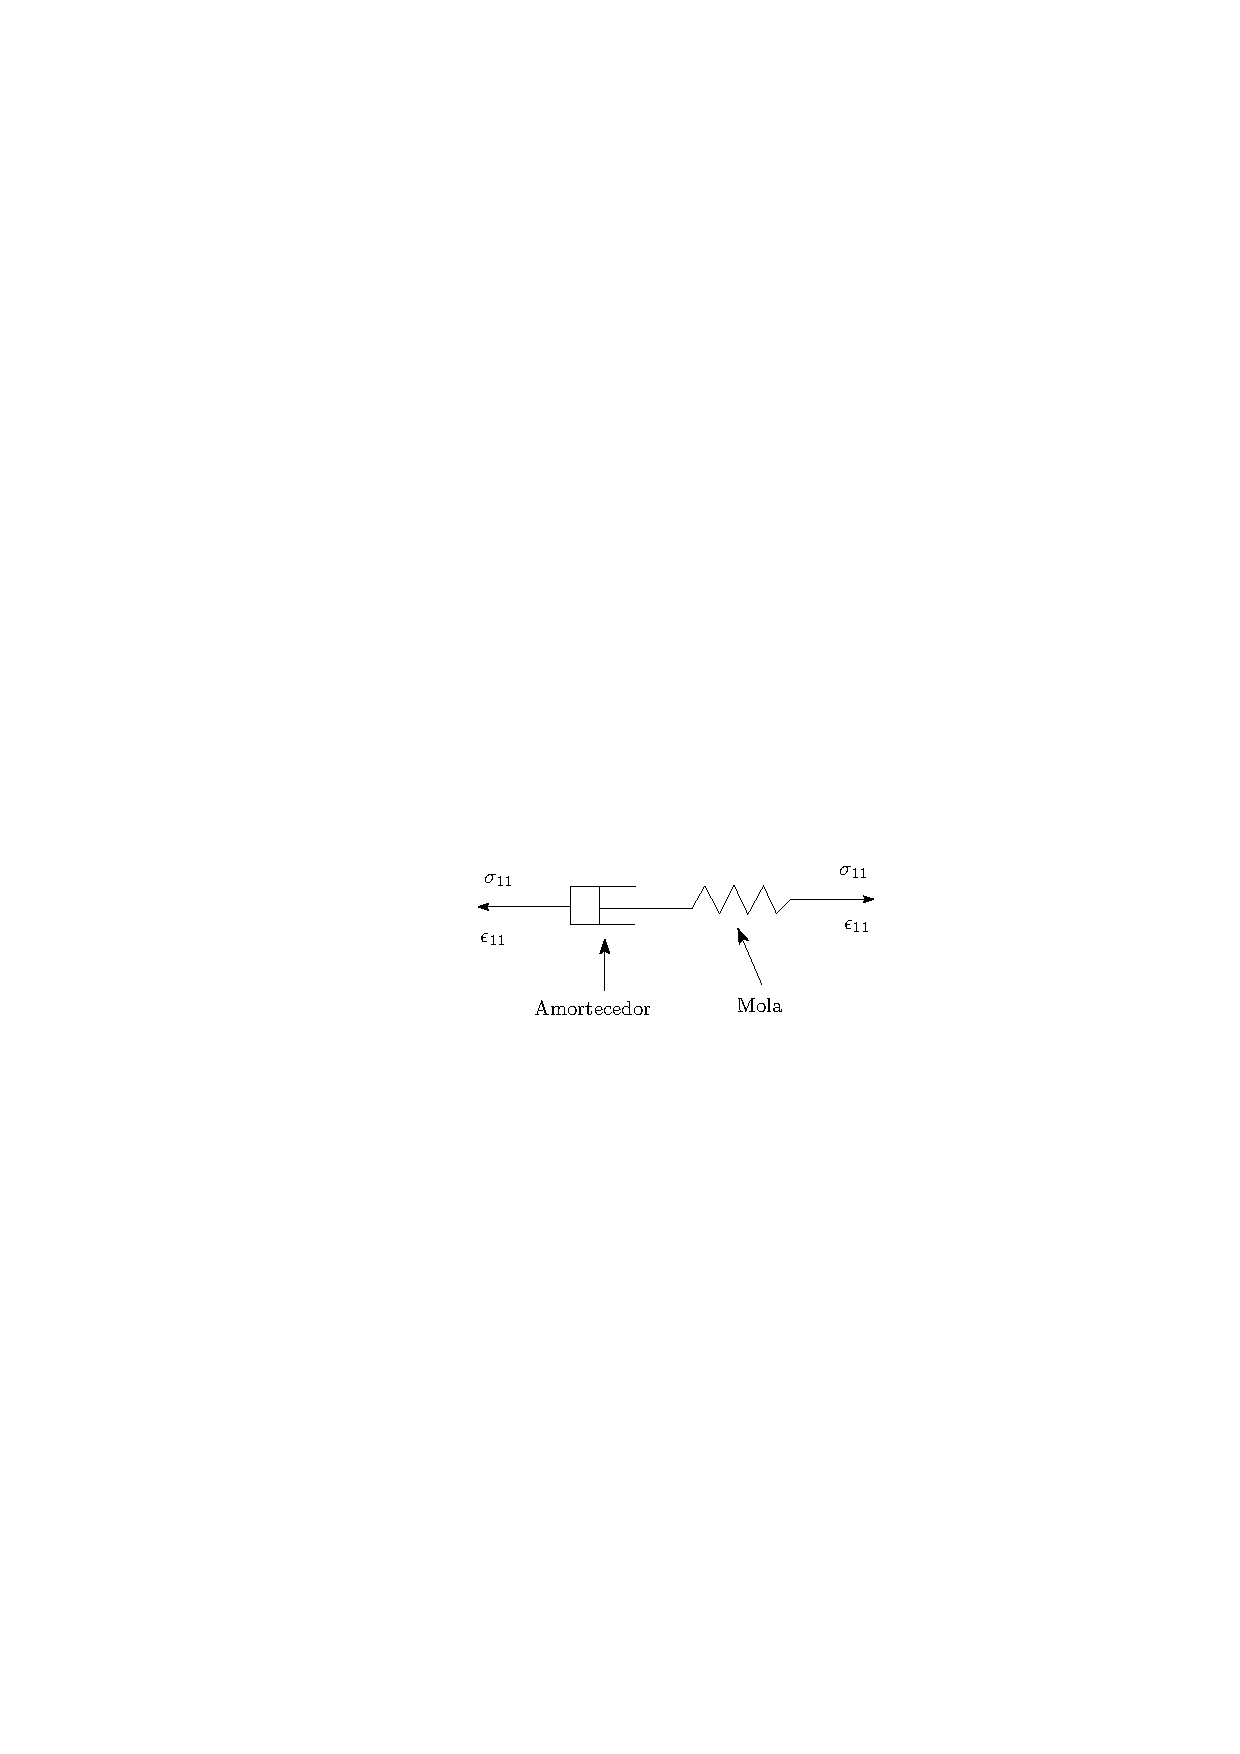
\includegraphics[scale=1.1]{images/maxwell}
			\end{figure}
			
			\begin{equation}
			\dfrac{\dot{\sigma}_{11}(M)}{E}+\dfrac{\sigma_{11}(A)}{\eta}=\dot{\epsilon}_{11}
			\end{equation}
			
			\item Modelo de Kelvin
			\begin{figure}[H]
				\centering
				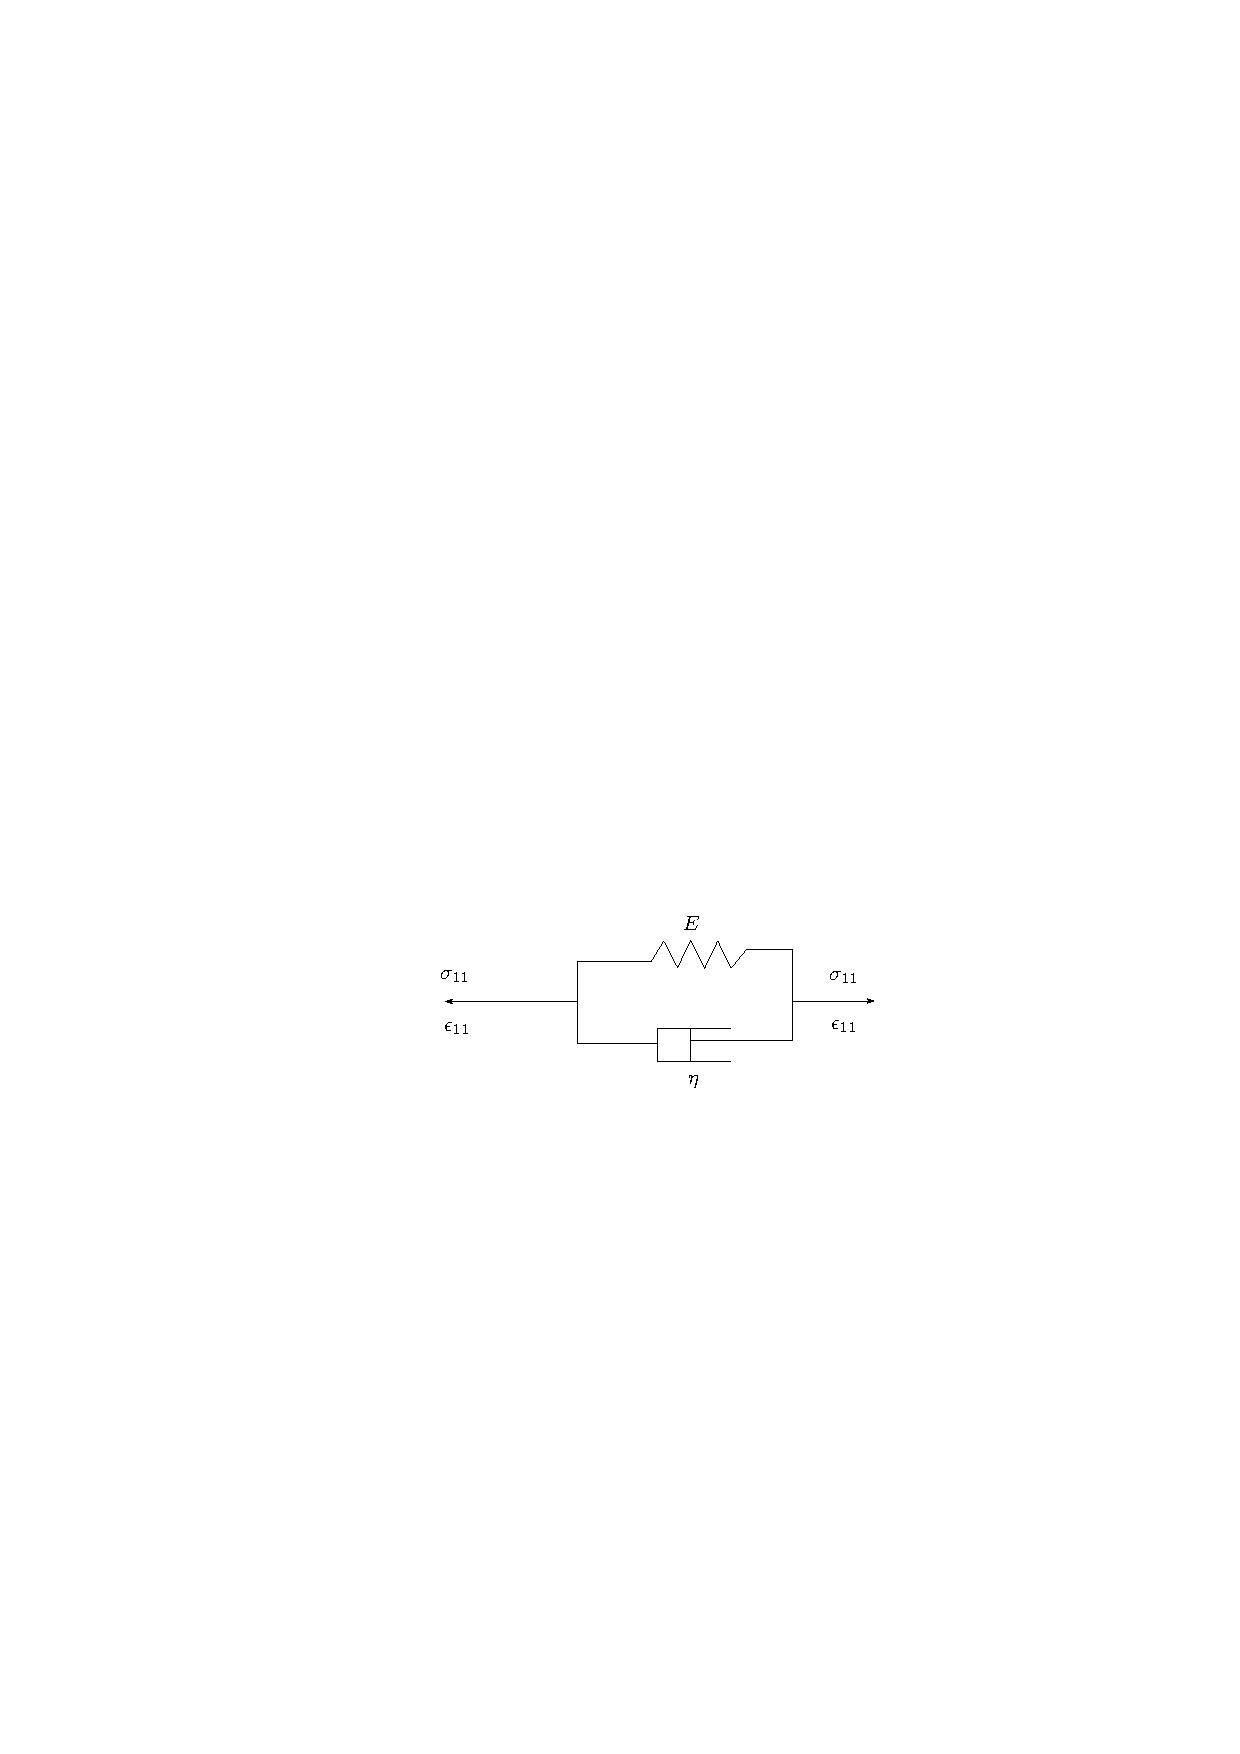
\includegraphics[scale=1.1]{images/kelvin}
			\end{figure}
			
			\begin{equation}
			\sigma_{11}(t)(T)=E\,\epsilon_{11}(t)(M)+\eta\,\dot{\epsilon}_{11}(t)(A)
			\end{equation}
		\end{itemize}
		
		
		\item[\textbf{(7)}] Para obtenção do módulo $E$ é necessário basear-se no ensaio de cargas de contato e determinação do módulo de firmeza do material. O módulo referido é o de elasticidade ou de Young. 
		
		Caso a área de contato não seja obtida é necessário lançar mão da literatura visando obter o módulo de firmeza do material estudado. Ao analisar a equação de Hertz abaixo
		
		\begin{equation}
			a=\sqrt[3]{\dfrac{3F(1-\nu^{2})\,R}{4E}}
		\end{equation}
		ao rearranjar os termos, temos que
		
		\begin{equation}
			\label{eq:hertz}
			\left(\dfrac{E}{1-\nu^{2}}\right)=\dfrac{3FR}{4a^{3}}
		\end{equation}
		dessa forma, por não possuirmos as características associadas à área de contato seria necessário aplicar somente o lado direito de \eqref{eq:hertz} visando obter o módulo $E$. Porém a consideração a ser feita seria
		
		\begin{equation}
			\textit{firmness}=\dfrac{E}{1-\nu^{2}}
		\end{equation}
		onde \textit{firmness} e $\nu$ são conhecidos.
	
		\item[\textbf{(8)}]		
		
		\begin{itemize}
			\item[\textbf{(a)}] A linearidade ou não linearidade geométrica estão vinculadas às características físicas do material ao ser submetido a esforços e solicitações. Sendo que estes podem originar deformações do material e a consequente alteração da sua estabilidade.
			\item[\textbf{(b)}] A linearidade material está vinculada às características dependentes do tempo, oriundas das mudanças físicas no interior do corpo afetando a sua uniformidade e semelhanças estruturais em toda sua porção, podendo ocasionar variação das propriedades mecânicas.
		\end{itemize}
	
		\item[\textbf{(9)}] As constante a serem obtidas dizem respeito aos módulos $E$, $\nu$ e $G$. A primeiro -- módulo de Young -- pode ser retirado da curva tensão ($\sigma$) \textit{versus} deformação ($\epsilon$) no trecho onde as duas grandezas de comportam de forma linear, onde a lei de Hooke é válida. Dessa forma, ao basear-se num determinado material devem ser feitos sucessivos ensaios visando analisar o comportamento da tensão em função da deformação. A figura \cref{fig:graph} ilustra o procedimento, onde após terem sido realizadas cinco repetições de compressão axial da batata inglesa, sob diferentes velocidades, foi ajustada uma reta que contempla a inclinação do trecho linear das cinco curvas permitindo, desta maneira, obter o módulo $E$ do material. Para $\nu$ -- coeficiente do Poisson -- ele é obtido da compressão axial sob restrição de corpos de prova, onde a partir das condições de contorno do experimento e fazendo uso da equação da elasticidade 
		
		\begin{equation}
			\dfrac{M}{E}=\dfrac{1-\nu}{(1+\nu)(1-2\nu)}
		\end{equation}
		
		sabendo que $M$ é o coeficiente angular do ensaio sob restrição e $E$ o módulo de elasticidade do mesmo material obtido na primeira parte, é possível calcular $\nu$. Por fim, tendo $E$ e $\nu$ em mãos é possíve calcular $G$ como função das duas primeiras.
		
		\begin{figure}[H]
			\centering
			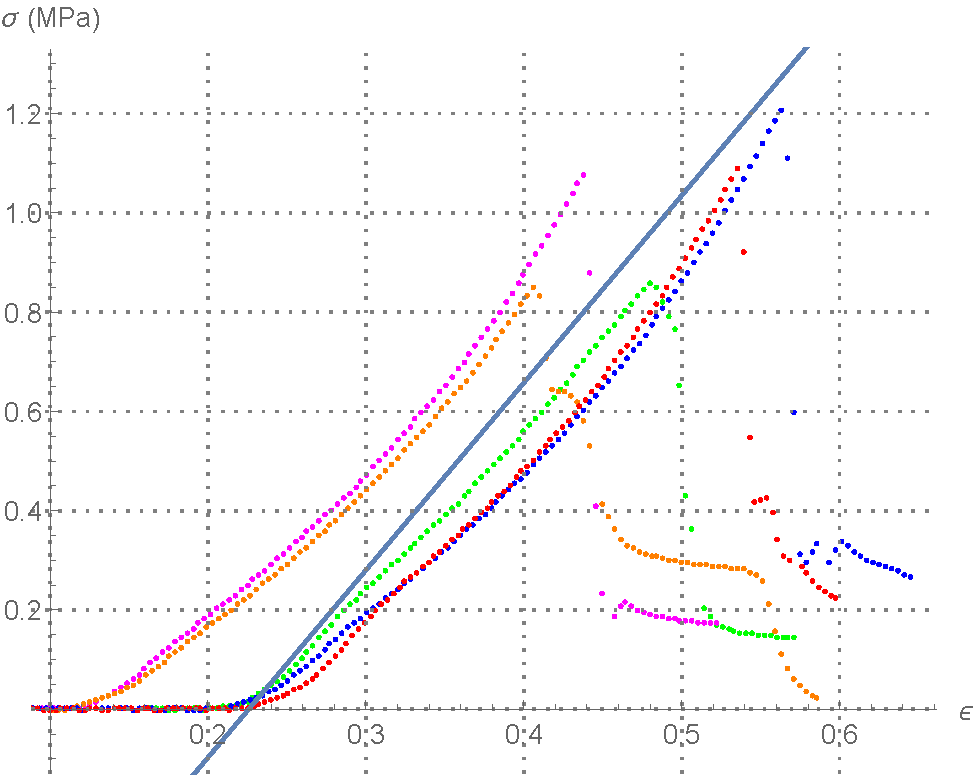
\includegraphics[scale=.6]{images/g3}
			\label{fig:graph}
		\end{figure} 	
	
		\item[\textbf{(10)}]
		
		\begin{equation}
			E=\dfrac{8(1-\nu^{2})Z^{2}F}{\pi D}
		\end{equation}
		
		\begin{equation}
			Z=\dfrac{R}{b}
		\end{equation}
		
		\begin{equation}
			\dfrac{D}{d}=\dfrac{1}{2Z^{2}}\left[\ln (2Z)+\dfrac{1}{2}\right]
		\end{equation}
		As três equações apresentadas acima referem-se ao ensaio de compressão diametral de um corpo de prova cilíndrico. $E$ e $\nu$ representam o módulo de Young e coeficiente de Poisson, respectivamente. $Z$ é uma grandeza adimensional dada pela razão entre o raio do cilindro ($R$) e a metade da largura da área de contato. $F$ é a força máxima aplicada na deformação do corpo de prova, enquanto $D$ e $d$ são a deformação e o diâmetro do cilindro, respectivamente.
		
		\item[\textbf{(11)}]
		
		\begin{equation}
			\mathscr{L}\{f(t)\}=\int\limits_{0}^{\infty}f(t)e^{-st}dt
		\end{equation}
		
		Sendo $\psi(t)$ a função \textit{creep} e $\phi(t)$ a função \textit{relaxation}
		
		\begin{equation}
			\therefore\psi(s)\phi(s)=\dfrac{1}{s^{2}}
		\end{equation} 
		
		
		\item[\textbf{(12)}] As perdas podem ser diminuídas a partir do estudo mais aprofundado envolvendo a interação das operações mecanizadas e os esforços suportados por cada material. Ou seja, deve-se haver mais especificidade e adequação entre o que o produto requer para que não sofra danos ou injúrias mecânicas e os elementos ao longo da cadeia de produção, englobando todas as variáveis pertinentes até a fase de comercializar a mercadoria.
	\end{itemize} 
\end{document}